\documentclass[dvipdfmx]{article}
\usepackage[dvipdfmx]{graphicx}
\usepackage[dvipdfmx]{hyperref}
\begin{document}

\section*{Transpose}
The arbitrary matrix $A$ is transposed to matrix $A^T$.\\
The example is shown as
\[
  A = \left(
    \begin{array}{ccc}
      1 & 2 & 3 \\
      4 & 5 & 6 \\
      7 & 8 & 9
    \end{array}
  \right) 
  , \ \ \
  A^T = \left(
    \begin{array}{ccc}
      1 & 4 & 7 \\
      2 & 5 & 8 \\
      3 & 6 & 9
    \end{array}
  \right) .
\] 


\section*{Trace}
The trace of a square matrix A (${\rm{tr}}A$) is defined to be the sum of elements on the main diagonal of A.
The example is shown as
\[
  A = 
  \left(
    \begin{array}{ccc}
      a_{11} & a_{12} & a_{13} \\
      a_{21} & a_{22} & a_{23} \\
      a_{31} & a_{32} & a_{33}
    \end{array}
  \right)  =
  \left(
    \begin{array}{ccc}
      1 & 2 & 3 \\
      4 & 5 & 6 \\
      7 & 8 & 9
    \end{array}
  \right) 
\] 
then \
${\rm{tr}}A =  {\sum_i}a_{ii} = 15$.


\section*{Determinant}
For a 3 × 3 matrix A, its determinant is \\
\[
  |A| = 
    \left|
    \begin{array}{ccc}
      a_{11} & a_{12} & a_{13} \\
      a_{21} & a_{22} & a_{23} \\
      a_{31} & a_{32} & a_{33}
    \end{array}
  \right| =
   a_{11}
  \left|
    \begin{array}{ccc}
      \times & \times & \times \\
      \times & a_{22} & a_{23} \\
      \times & a_{32} & a_{33}
    \end{array}
  \right|  
  - a_{12}
  \left|
    \begin{array}{ccc}
      \times & \times & \times \\
      a_{21} & \times & a_{23} \\
      a_{31} & \times & a_{33}
    \end{array}
  \right| 
  + a_{13}
    \left|
    \begin{array}{ccc}
      \times & \times & \times \\
      a_{21} & a_{22} & \times \\
      a_{31} & a_{32} & \times
    \end{array}
  \right|
\] 
\[
   = a_{11}
     \left|
    \begin{array}{ccc}
      a_{22} & a_{23} \\
      a_{32} & a_{33}
    \end{array}
  \right|  
  - a_{12}
  \left|
    \begin{array}{ccc}
      a_{21} & a_{23} \\
      a_{31} & a_{33}
    \end{array}
  \right| 
  + a_{13}
    \left|
    \begin{array}{ccc}
      a_{21} & a_{22}  \\
      a_{31} & a_{32} 
    \end{array}
  \right|
\] 
\[
  \ \ \ \ \ \ = a_{11} a_{22}
     \left|
    \begin{array}{ccc}
      \times & \times \\
      \times & a_{33}
    \end{array}
  \right|  
  - a_{11} a_{23}
     \left|
    \begin{array}{ccc}
      \times & \times \\
      a_{32} & \times
    \end{array}
  \right|  
  - a_{12} a_{21}
  \left|
    \begin{array}{ccc}
      \times & \times \\
      \times & a_{33}
    \end{array}
  \right| 
   \] 
 \[
   \ \ \ \ \ \ + a_{12} a_{23}
  \left|
    \begin{array}{ccc}
      \times & \times \\
      a_{31} & \times
    \end{array}
  \right| 
  + a_{13} a_{21}
    \left|
    \begin{array}{ccc}
      \times & \times \\
      \times & a_{32} 
    \end{array}
  \right|
    - a_{13} a_{22}
    \left|
    \begin{array}{ccc}
      \times & \times \\
      a_{31} & \times 
    \end{array}
  \right|
\]
\ \ \ \ \ = $a_{11}a_{22}a_{33} - a_{11}a_{23}a_{32} - a_{12}a_{21}a_{33} + a_{12}a_{23}a_{31} + a_{13}a_{22}a_{31}$


\section*{Cramer's rule}
In a system of $n$ linear equations, represented in matrix multiplication form
$A{\bf{x}} = {\bf{b}}$ \\
where $A$ is the $n {\times} n$ matrix and {\bf{x}} and {\bf{b}} are the $n$-th column vectors.
${\bf{x}} = (x_1, {\cdots}, x_n)^T$ , ${\bf{b}} = (b_1, {\cdots}, b_n)^T$. \\
Then, if $|A| {\neq} 0$,  \\
 \[
   x_i = |A_i| / |A|, \ \ \ 
   A_i =
   \left(
   \begin{array}{ccccc}
   a_{11} & \cdots & b_{1i} & \cdots & a_{1n} \\
   \vdots & \ddots  & \vdots & 	     &  \vdots \\
   a_{k1} &             & b_{ki} &           & a_{kn} \\
   \vdots &            & \vdots & \ddots  &  \vdots \\
   a_{n1} & \cdots & b_{ni} & \cdots &  a_{nn}
   \end{array}
   \right)
   \]
This is Cramer's rule.


\section*{LU decomposition}
$A = LU$ where
 \[
   A =
   \left(
   \begin{array}{ccc}
   a_{11} & a_{12} & a_{13} \\
   a_{21} & a_{22} & a_{23} \\
   a_{31} & a_{32} & a_{33} 
   \end{array}
   \right) ,
    L =
   \left(
   \begin{array}{ccc}
   1 & 0 & 0 \\
   l_{21} & 1 & 0 \\
   l_{31} & l_{32} & 1 
   \end{array}
   \right) ,
     U =
   \left(
   \begin{array}{ccc}
   u_{11} & u_{12} & u_{13} \\
   0         & u_{22} & u_{23} \\
   0         & 0         & u_{33} 
   \end{array}
   \right) 
  \]


\section*{Direct method by LU decomposition}
In linear equation $A{\bf{x}} = {\bf{b}}$, 
$LU{\bf{x}} = {\bf{b}}$
by using LU decomposition $A = LU$.

Here, we consider $L{\bf{y}} = {\bf{b}}$ and $U{\bf{x}} = {\bf{y}}$.

In forward substitution,
\begin{eqnarray}
y_1 &&= b_1 \nonumber \\
y_2 &&= b_2 - l_{21}y_1 \nonumber \\
{\vdots} \nonumber \\
y_n &&= b_n - {\sum_{j=1}^{n-1}} l_{nj}y_j \nonumber 
\end{eqnarray}

In backforward substitution,
\begin{eqnarray}
x_n &&= y_n / u_{nn} \nonumber \\ 
x_{n-1} &&= (y_{n-1} - u_{n-1, n}x_n) / u_{n-1, n-1} \nonumber \\ 
{\vdots} \nonumber \\
x_1 &&= (y_1 - {\sum_{j=2}^{n}} u_{1, j}x_j) / u_{11} \nonumber 
\end{eqnarray} .


\section*{Constant multiple}
 \[
   c
   \left(
   \begin{array}{ccc}
   a_{11} & \cdots & a_{1n} \\
   \vdots & \ddots  & \vdots \\
   a_{n1} & \cdots & a_{nn}
   \end{array}
   \right)
   =
   \left(
   \begin{array}{ccc}
   ca_{11} & \cdots & ca_{1n} \\
   \vdots & \ddots  & \vdots \\
   ca_{n1} & \cdots & ca_{nn}
   \end{array}
   \right)
   \]
where $c$ is the scalar constant.


\section*{Inverse matrix}
$AB = BA = I$ \\
where $A$ and $B$ is the $n$ × $n$ matrices and $I$ is the $n$ × $n$ unit matrix.
In the case, the matrix $B$ is uniquely determined by $A$ and is called the inverse matrix of $A$.
The inverse matrix of $A$ is denoted by $A^{-1}$.


\section*{Product}
The elements of the matrix product $C = AB$ is that
$c_{ij} = [AB]_{ij} = {\sum_k}a_{ik}b_{kj}$ 
where $A$ is an $n \times m$ matrix and $B$ is an $m \times l$  matrix.


\section*{Addition and Subtraction}
 \[
   A=
   \left(
   \begin{array}{ccc}
   a_{11} & a_{12} & a_{13} \\
   a_{21} & a_{22}  & a_{23} \\
   a_{31} & a_{32} & a_{33}
   \end{array}
   \right) ,
   B =
   \left(
   \begin{array}{ccc}
   b_{11} & b_{12} & b_{13} \\
   b_{21} & b_{22}  & b_{23} \\
   b_{31} & b_{32} & b_{33}
   \end{array}
   \right) ,
 \]
then the addition/subtraction is that
 \[
   A {\pm} B=
   \left(
   \begin{array}{ccc}
   a_{11}  {\pm} b_{11} & a_{12}  {\pm} b_{12}  & a_{13}  {\pm} b_{13} \\
   a_{21}  {\pm} b_{21} & a_{22}  {\pm} b_{22} & a_{23}  {\pm} b_{23} \\
   a_{31}  {\pm} b_{31} & a_{32}  {\pm} b_{32} & a_{33}  {\pm} b_{33}
   \end{array}
   \right) 
 \]


\section*{Hadamard product}
 \[
   A=
   \left(
   \begin{array}{ccc}
   a_{11} & a_{12} & a_{13} \\
   a_{21} & a_{22}  & a_{23} \\
   a_{31} & a_{32} & a_{33}
   \end{array}
   \right) ,
   B =
   \left(
   \begin{array}{ccc}
   b_{11} & b_{12} & b_{13} \\
   b_{21} & b_{22}  & b_{23} \\
   b_{31} & b_{32} & b_{33}
   \end{array}
   \right) ,
 \]
then the Hadamard product is that
 \[
   A {\circ} B=
   \left(
   \begin{array}{ccc}
   a_{11} b_{11} & a_{12} b_{12}  & a_{13} b_{13} \\
   a_{21} b_{21} & a_{22} b_{22} & a_{23} b_{23} \\
   a_{31} b_{31} & a_{32} b_{32} & a_{33} b_{33}
   \end{array}
   \right) 
 \]


\section*{Hadamard division}
 \[
   A=
   \left(
   \begin{array}{ccc}
   a_{11} & a_{12} & a_{13} \\
   a_{21} & a_{22}  & a_{23} \\
   a_{31} & a_{32} & a_{33}
   \end{array}
   \right) ,
   B =
   \left(
   \begin{array}{ccc}
   b_{11} & b_{12} & b_{13} \\
   b_{21} & b_{22}  & b_{23} \\
   b_{31} & b_{32} & b_{33}
   \end{array}
   \right) ,
 \]
then the Hadamard division is that
 \[
   A / B=
   \left(
   \begin{array}{ccc}
   a_{11} / b_{11} & a_{12} / b_{12}  & a_{13} / b_{13} \\
   a_{21} / b_{21} & a_{22} / b_{22} & a_{23} / b_{23} \\
   a_{31} / b_{31} & a_{32} / b_{32} & a_{33} / b_{33}
   \end{array}
   \right) 
 \]


\section*{Hadamard power}
 \[
   A^{(n)}=
   \left(
   \begin{array}{ccc}
   a_{11}^n & a_{12}^n & a_{13}^n \\
   a_{21}^n & a_{22}^n  & a_{23}^n \\
   a_{31}^n & a_{32}^n & a_{33}^n
   \end{array}
   \right)
 \]
 where $n$ is scalar.


\section*{Tensor product}
 \[
   A=
   \left(
   \begin{array}{ccc}
   a_{11} & a_{12} & a_{13} \\
   a_{21} & a_{22}  & a_{23} \\
   a_{31} & a_{32} & a_{33}
   \end{array}
   \right) ,
   B =
   \left(
   \begin{array}{ccc}
   b_{11} & b_{12} & b_{13} \\
   b_{21} & b_{22}  & b_{23} \\
   b_{31} & b_{32} & b_{33}
   \end{array}
   \right) ,
 \]
then the tensor product is that
 \[
   A {\otimes} B =
   \left(
   \begin{array}{ccc}
   a_{11} B & a_{12} B  & a_{13} B \\
   a_{21} B & a_{22} B & a_{23} B \\
   a_{31} B & a_{32} B & a_{33} B
   \end{array}
  \right)
\]
\[
    =
   \left(
   \begin{array}{ccccccccc}
   a_{11} b_{11} & a_{11} b_{12} & a_{11} b_{13} & a_{12} b_{11} & a_{12} b_{12} & a_{12} b_{13} & a_{13} b_{11} & a_{13} b_{12} & a_{13} b_{13} \\
   a_{11} b_{21} & a_{11} b_{22} & a_{11} b_{23} & a_{12} b_{21} & a_{12} b_{22} & a_{12} b_{23} & a_{13} b_{21} & a_{13} b_{22} & a_{13} b_{23} \\
   a_{11} b_{31} & a_{11} b_{32} & a_{11} b_{33} & a_{12} b_{31} & a_{12} b_{32} & a_{12} b_{33} & a_{13} b_{31} & a_{13} b_{32} & a_{13} b_{33} \\
   a_{21} b_{11} & a_{21} b_{12} & a_{21} b_{13} & a_{22} b_{11} & a_{22} b_{12} & a_{22} b_{13} & a_{23} b_{11} & a_{23} b_{12} & a_{23} b_{13} \\
   a_{21} b_{21} & a_{21} b_{22} & a_{21} b_{23} & a_{22} b_{21} & a_{22} b_{22} & a_{22} b_{23} & a_{23} b_{21} & a_{23} b_{22} & a_{23} b_{23} \\
   a_{21} b_{31} & a_{21} b_{32} & a_{21} b_{33} & a_{22} b_{31} & a_{22} b_{32} & a_{22} b_{33} & a_{23} b_{31} & a_{23} b_{32} & a_{23} b_{33} \\
   a_{31} b_{11} & a_{31} b_{12} & a_{31} b_{13} & a_{32} b_{11} & a_{32} b_{12} & a_{32} b_{13} & a_{33} b_{11} & a_{33} b_{12} & a_{33} b_{13} \\
   a_{31} b_{21} & a_{31} b_{22} & a_{31} b_{23} & a_{32} b_{21} & a_{32} b_{22} & a_{32} b_{23} & a_{33} b_{21} & a_{33} b_{22} & a_{33} b_{23} \\
   a_{31} b_{31} & a_{31} b_{32} & a_{31} b_{33} & a_{32} b_{31} & a_{32} b_{32} & a_{32} b_{33} & a_{33} b_{31} & a_{33} b_{32} & a_{33} b_{33}
   \end{array}
   \right) 
 \]


\section*{Eigenvalue (Algebraic method)}
An eigen equation is written as
$A{\bf{u}} = {\lambda}{\bf{u}}$ 
where ${\lambda}$ is scalar and ${\bf{u}}$ is vector, known as the eigenvalue and eigenvector.

By rearranging above equation, we obtain:  $A{\bf{u}} = {\lambda}{\bf{u}}$, $(A - {\lambda}I){\bf{u}} = {\bf{0}}$. 
If this equation has a nontrivial solution (${\bf{u}} {\neq} 0$),
the determinant $|A - {\lambda}I| = 0$.

\begin{flushleft}
[$2 {\times} 2$ matrix case] 
\end{flushleft}
When the matrix $A$ is written as
 \[
   A=
   \left(
   \begin{array}{cc}
   a_{11} & a_{12}  \\
   a_{21} & a_{22} \\
   \end{array}
   \right) ,
  \]
the quadratic equation ${\lambda}^2 -(a_{11} - a_{22}){\lambda} + a_{11}a_{22} - a_{12}a_{21}$ is obtained.
By using quadratic formula, 
\begin{eqnarray}
{\lambda} =  \frac{ a_{11} -a_{22} {\pm} \sqrt{(a_{11}-a_{22})^2 - 4(a_{11}a_{22} - a_{12}a_{21})} }{2}. \nonumber
\end{eqnarray} \\

\begin{flushleft}
[$3 {\times} 3$ matrix case]
\end{flushleft}
When the matrix $A$ is written as
 \[
   A=
   \left(
   \begin{array}{ccc}
   a_{11} & a_{12} & a_{13} \\
   a_{21} & a_{22} & a_{23} \\
   a_{31} & a_{32} & a_{33} \\
   \end{array}
   \right) ,
  \]
we obtain the cubic equation $a{\lambda}^3 + b{\lambda}^2 + c{\lambda} + d = 0$  where \\
$a = -1$, \\
$b = a_{11} + a_{22} + a_{33}$, \\
$c = a_{21}a_{12} + a_{13}a_{31} + a_{32}a_{23} - a_{11}a_{22} - a_{11}a_{33} - a_{22}a_{33}$, \\
$d =  a_{11}a_{22}a_{33} + a_{12}a_{23}a_{31} + a_{13}a_{32}a_{21} - a_{11}a_{32}a_{23} - a_{22}a_{31}a_{13} - a_{33}a_{21}a_{12}$ . \\

Therefore, 
we can solve the eigen equation in the case of the $3{\times}3$ matrix $A$ by substituting above $a$, $b$, $c$ and $d$ for the cubic formula.
The cubic formula is that 
\begin{eqnarray}
{\lambda}_1 &&= -\frac{b}{3a} \nonumber \\
       &&- \frac{1}{3a} \sqrt[3]{ \frac{1}{2} (2b^3 -9abc + 27a^2d + \sqrt{(ab^3) - 9abc + 27a^2d)^2 - 4(b^2 - 3ac)^3} ) } \nonumber \\  
       &&- \frac{1}{3a} \sqrt[3]{ \frac{1}{2} (2b^3 -9abc + 27a^2d - \sqrt{(ab^3) - 9abc + 27a^2d)^2 - 4(b^2 - 3ac)^3} ) } \ \ \ , \nonumber \\ 
\nonumber \\
{\lambda}_2 &&= -\frac{b}{3a} \nonumber \\
       &&- \frac{1 + i \sqrt{3}}{6a} \sqrt[3]{ \frac{1}{2} (2b^3 -9abc + 27a^2d + \sqrt{(ab^3) - 9abc + 27a^2d)^2 - 4(b^2 - 3ac)^3} ) } \nonumber \\  
       &&- \frac{1 - i \sqrt{3}}{6a} \sqrt[3]{ \frac{1}{2} (2b^3 -9abc + 27a^2d - \sqrt{(ab^3) - 9abc + 27a^2d)^2 - 4(b^2 - 3ac)^3} ) } \ \ \ , \nonumber \\ 
\nonumber \\
{\lambda}_3 &&= -\frac{b}{3a} \nonumber \\
       &&- \frac{1 - i \sqrt{3}}{6a} \sqrt[3]{ \frac{1}{2} (2b^3 -9abc + 27a^2d + \sqrt{(ab^3) - 9abc + 27a^2d)^2 - 4(b^2 - 3ac)^3} ) } \nonumber \\  
       &&- \frac{1 + i \sqrt{3}}{6a} \sqrt[3]{ \frac{1}{2} (2b^3 -9abc + 27a^2d - \sqrt{(ab^3) - 9abc + 27a^2d)^2 - 4(b^2 - 3ac)^3} ) } \ \ \ . \nonumber 
\end{eqnarray}
 
In this Elixir library, the complex numbers in the above equations are calculated as Gaussian plane.
\begin{center}
  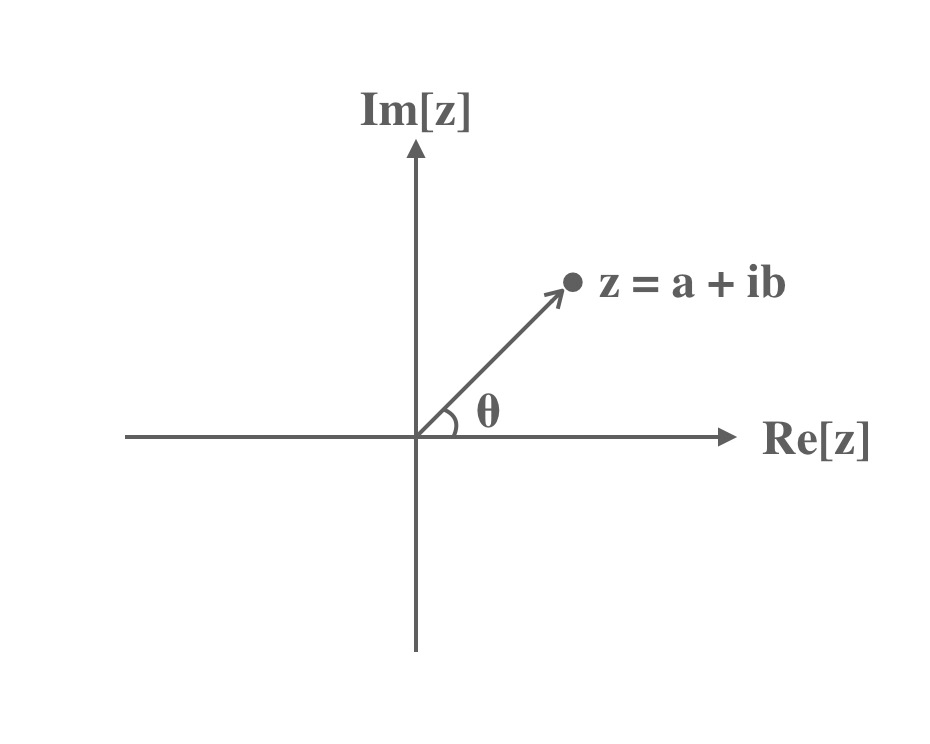
\includegraphics[width=10cm]{gaussian_plane.jpg}
\end{center}

The real part and imaginary part are calculated by using arctangent's integral formula, written as
 \begin{eqnarray}
 \arctan{x} = {\int_0^x} \frac{1}{z^2 + 1} dz. \nonumber
 \end{eqnarray}
 This formula is treated as the numerical integration.


\section*{Eigenvalue and eigenvector (Power iteration method to solve maximum eigenvalue and eigenvector of $n$-th eigen equation)}
An arbitrary (initial) vector ${\bf{b}}^0$ is written by the linear combination of eigenvectors ${\sum_i} c_i{\bf{u}}_i$
because eigenvectors are linearly independent.
\begin{eqnarray}
{\bf{b}}^k {\equiv} A^k {\bf{b}}^0 = A^k {\sum_i} c_i{\bf{u}}_i = {\sum_{i=1}} c_i {\lambda}^k_i {\bf{u}}_i \nonumber \\
= {\lambda}_1^k (c_1{\bf{u}}_1 + {\sum_{i=2}} c_i \frac{{\lambda}^k_i}{{\lambda}^k_1} {\bf{u}}_i)  \nonumber
\end{eqnarray}
where ${\lambda}_1$ is maximum value of the eigenvalue so that $|\frac{{\lambda}^k_i}{{\lambda}^k_1}| < 1$.

If $k$ is a large enough number, 
we can write the eigenvector of the maximum eigenvalue, shown as
\begin{eqnarray}
{\bf{b}}^k {\simeq} {\lambda}^k_1c_1{\bf{u}}_1. \nonumber
\end{eqnarray} 
Moreover,  we can write the maximum eigenvalue
\begin{eqnarray}
{\lambda}_1 = \frac{({\bf{b}}^k)^TA{\bf{b}}^k}{({\bf{b}}^k)^T{\bf{b}}^k}. \nonumber
\end{eqnarray}


\section*{Eigenvalue and eigenvector (Jacobi method)}
The Jacobi method is an iterative method for the numerical calculation of the eigenvalues and eigenvectors of a real $n$-th symmetric matrix.
(cf. \url{https://en.wikipedia.org/wiki/Jacobi_eigenvalue_algorithm} )


\section*{Eigenvalue (iterative method using QR decomposition)}
The iterative method using QR decomposition is used to calculate eigenvalues of a $n$-th real square matrix.
The QR decomposition is the decomposition of matrix $A$ into orthogonal matrix $Q$ and upper-triangular matrix $R$ as shown below.
$$
A = QR
$$
In this section, QR decomposition is performed by using Householder transformation.
Householder transformation corresponds to matrix $H$ below. 
\begin{eqnarray}
{\bf{x}} = H {\bf{y}} \nonumber \\
{\bf{y}} = H {\bf{x}} \nonumber
\end{eqnarray}
\begin{eqnarray}
H = I - \frac{2({\bf{x}} - {\bf{y}})({\bf{x}} - {\bf{y}})^T}{|{\bf{x}} - {\bf{y}}|^2} \nonumber
\end{eqnarray}
$H$ is orthogonal matrix where $HH^T=I$.
Here,
\[
  A = A^{(1)} =
  \left(
  \begin{array}{ccc}
  a_{11} & \cdots & a_{1n} \\
  \vdots & \ddots & \vdots \\
  a_{n1} & \cdots & a_{nn}
  \end{array}
  \right),
\]
$$
A^{(2)}=H^{(1)}A^{(1)}, \\
A^{(2)} =
\left(
\begin{array}{cccc}
a_{11} & a_{12} & \cdots & a_{1n} \\
0      & \vdots & \vdots & \vdots \\
\vdots & \vdots & \vdots & \vdots \\
0      & a_{n2} & \cdots & a_{nn}
\end{array}
\right).
$$
$H^{(1)}$ to Householder transform the first column into a finite vector with only the top element.

$$
A^{(3)}=H^{(2)}A^{(2)}, \\
A^{(3)} =
\left(
\begin{array}{ccccc}
a_{11} & a_{12} & a_{12} & \cdots & a_{1n} \\
0      & a_{22} & \vdots & \vdots & \vdots \\
0      & 0      & \vdots & \vdots & \vdots \\
\vdots & \vdots & \vdots & \vdots & \vdots \\
0      & 0      & a_{n2} & \cdots & a_{nn}
\end{array}
\right).
$$
$H^{(2)}$ to Householder transform the second column into a finite vector with the top 2 elements.

$$
H^{(n-1)} {\cdots} H^{(1)} A^{(1)} = R,
$$
$$
A = A^{(1)} = H^{(n-1)T} {\cdots} H^{(1)T} R = QR.
$$
The product of orthogonal matricies $Q_1$ and $Q_2$ is also orthogonal matrix $Q_3(=Q_1Q_2)$.


\section*{Rank}
Since the rank of matrix is equal to the number of nontrivial nonzero eigenvalues, 
it is calculated from the eigenvalues obtained by the Jacobi method or iterative method using QR decomposition.
In this library, we use iterative method using QR decomposition, which has a faster processing speed.

 
\section*{Singular Value Decomposition}
Singular value decomposition (SVD) states:
$$
A = U {\Sigma} V^T
$$
where $A$ and ${\Sigma}$ is ${n{\times}m}$ matrix, $U$ is ${n{\times}n}$ orthogonal matrix, $U$ is ${m{\times}m}$ orthogonal matrix.
In the case $m > n$,
 \[
   {\Sigma} =
   \left(
   \begin{array}{ccc|c}
   {\sigma}_{11} & \            & O                    & \ \\
   \                      & {\ddots} & \                     & O \\
   O                    & \            & {\sigma}_{nn} & \
   \end{array}
   \right) 
  \] 
  where ${\sigma}$ is singular value.

It can be replaced by an eigenvalue problem from the following relation.
$$
AA^T = U {\Sigma} V^T  (U {\Sigma} V^T)^T = U{\Sigma}^2U^T ,
$$
 \[
   {\Sigma}^2 =
   \left(
   \begin{array}{ccc}
   {\sigma}_{11}^2 & \            & O \\
   \                         & {\ddots} & \   \\
   O                       & \            & {\sigma}_{nn}^2
   \end{array}
   \right) =
   \left(
   \begin{array}{ccc}
   {\lambda}_{11} & \            & O \\
   \                       & {\ddots} & \   \\
   O                     & \            & {\lambda}_{nn}
   \end{array}
   \right) 
  \] 
  where $\lambda$ is eigenvalue of $AA^T$.
 

\section*{Diagonalization}
An $n{\times}n$ matrix $A$ is diagonalizable when $A$ has $n$ eigenvectors that are linear independent of each other.
We consider the matrix $P$ that is written as $P=[{\bf{x}}_1, {\bf{x}}_2, {\cdots}, {\bf{x}}_n]$ where ${\bf{x}}_i, i=1,{\cdots},n$ linear independent eigenvector of $A$.

\begin{eqnarray}
AP = A[{\bf{x}}_1, {\bf{x}}_2, {\cdots}, {\bf{x}}_n]
     = [{\lambda}_1{\bf{x}}_1, {\lambda}_2{\bf{x}}_2, {\cdots}, {\lambda}_n{\bf{x}}_n] \nonumber
\end{eqnarray}
where ${\lambda}_i, i=1,{\cdots},n$ eigenvalue of $A$.
Since ${\bf{x}}_1, {\bf{x}}_2, {\cdots}, {\bf{x}}_n$ are linear independent,
\[
  P^{-1}AP =
  \left(
  \begin{array}{ccc}
  {\lambda}_{1} & \ & O \\
  \          & \ddots  & \    \\
  O        &   \          & {\lambda}_{n}
  \end{array}
  \right)
\] .
This matrix is the diagonal matrix of $A$.
 
 
\section*{Jordan normal form}
Since $(A - {\lambda}E){\bf{u}} = {\bf{x}}$ and $(A - {\lambda}E){\bf{x}} = {\bf{0}}$,
\begin{eqnarray}
\left\{ \begin{array}{ll}
A{\bf{u}}= {\bf{x}} + {\lambda}{\bf{u}} \\
A{\bf{x}}={\lambda}{\bf{x}} \\
\end{array} \right.
\end{eqnarray} .

Therefore,
 \[
   A
   \left(
   \begin{array}{cc}
   {\bf{x}} & {\bf{u}} 
   \end{array}
   \right)
   =
   \left(
   \begin{array}{cc}
   {\bf{x}} & {\bf{u}} 
   \end{array}
   \right)
   \left(
   \begin{array}{cc}
   {\lambda} & 1 \\
   0 & {\lambda}
   \end{array}
   \right)
  \] .

$$P^{-1}AP = J$$ where
\[
   P =
   \left(
   \begin{array}{cc}
   {\bf{x}} & {\bf{u}} 
   \end{array}
   \right) ,
   J =
   \left(
   \begin{array}{cc}
   {\lambda} & 1 \\
   0 & {\lambda}
   \end{array}
   \right).
  \] .


\section*{Matrix norms}
$A$ is $n{\times}m$ matrix.

Frobenius norm:
$$
||A||_F = \sqrt{{\sum_i^n}{\sum_j^m} |a_{ij}|^2} \ \ .
$$
 
$L_1$ norm:
$$
||A||_1 = \max_{j}  {\sum_i^n} |a_{ij}| \ \ .
$$

Max norm:
$$
||A||_{\infty} = \max_{i}  {\sum_j^n} |a_{ij}| \ \ .
$$

$L_2$ norm:
$$
||A||_2 = \max_{ij}  {\sigma}_{ij}
$$
where $\sigma$ is singular value of $A$.


\section*{Variance covariance matrix}
A variance covariance matrix can be defined as
 \[
   S =
   \left(
   \begin{array}{cc}
   s_{xx} & s_{xy} \\
   s_{yx} & s_{yy}  
   \end{array}
   \right) 
  \]
where $s_{xx}$ is variance value and $s_{xy}$ is covariance value.
$s_{xy} = \frac{1}{n}({\bf{x}} - \bar{\bf{x}})({\bf{y}} - \bar{\bf{y}})$, $\bar{\bf{x}} = {\sum_{i=1}^n} x_i /n$.

By the way, we can consider the Principal Component Analysis (PCA) by this variance covariance matrix with above power Iteration library.

\end{document}